\documentclass[a4paper,12pt]{report}

\usepackage[utf8]{inputenc}
\usepackage[frenchb]{babel}
\usepackage[utf8]{inputenc}
\usepackage[T1]{fontenc}
\usepackage{geometry}
\usepackage{fancyhdr}
\usepackage{pdfpages}
\usepackage{hyperref}
\usepackage{pgf,tikz}
\usepackage{amsmath}
\usepackage{algorithm}
\usepackage{algorithmic}
\usetikzlibrary{arrows}

%Initialisation des entêtes et pieds de page
\pagestyle{fancy}
\renewcommand{\headrulewidth}{1pt}
\fancyhead[C]{}
\fancyhead[L]{MCS}
\fancyhead[R]{Rapport projet}
\renewcommand\footrulewidth{1pt}
\fancyfoot[C]{M1 Informatique - Université Paul Sabatier\\
\textbf{\thepage}}

\makeatletter
\renewcommand{\@chapapp}{}
\makeatother

%Faire dépendre les sections des partie pour avoir une numérotation à partir de 1
\makeatletter\@addtoreset{section}{part}\makeatother
\renewcommand{\thesection}{\arabic{section}}

\title{\LARGE \textbf{RAPPORT PROJET\\ Modélisation et Calcul Scientifique}}
\author{\textsc{Broders Nicolas -- Caussé Emmanuel }\\
\textsc{Courdy-Bahsoun Clémence -- Cousin Vincent}\\\\
M1 IHM -- M1 SIAME -- M1 IGAI -- M1 DC  \\
}
\date{23.11.2018}


\begin{document}
\maketitle
\newpage

\part*{Rapport}
\section{Application d'enregistrement de commande vocale}
\paragraph{Justification d'implémentation:\\}
Le choix d’extension de classe entre \textit{AudioRecord} et \textit{MediaRecorder} pour l’enregistrement se justifie par l’exigence que l’audio enregistré soit au format \textbf{WAV}. En effet, même si \textit{MediaRecorder} permet d’enregistrer des fichiers audio sous plusieurs format assez rapidement, il n’intègre pas dans ces méthodes l’enregistrement au format WAV. Il aura donc fallu partir de la classe \textit{AudioRecord} et de faire quelque modification (ajout d’un \textsc{en-tête wav}) pour obtenir le dit format.
\paragraph{Optimisation possible:\\}
Même si la seule exigence d’enregistrer au format WAV à été remplie, il existe des améliorations pour rendre plus agréable la navigation au sein même de l’application, à savoir:\\
Côté technique :
-- A la fin d’un enregistrement, armer le lecteur audio sur le dernier audio enregistrer.
-- Si on accède à la liste des audios enregistrés, armer le lecteur audio sur le premier enregistrement.\\
Côté graphique :
-- La possibilité de visualiser la force de la voix lors de l’enregistrement avec une courbe permettrait à l’utilisateur d’avoir un feed-back en direct et lui permettrait de s’ajuster.
(Les smartphones n’ont pas la même sensibilités au niveau du micro)
 Pour plus d'information le \hyperref[chap:Manuel]{Manuel Utilisateur} est disponible en Annexe.\\
 
 \newpage
\section{ DTW sans ACP}
\paragraph{}
Cette partie correspond aux résultats obtenus en terme de taux de reconnaissance par l'implémentation de la méthode DTW dans la première partie du TP. Dans laquelle on a pu constater que l'enregistrement de la base d'apprentissage avait un effet favorable sur la reconnaissance vocale.


\paragraph{Résultats:\\}
 Matrice de confusion sur un jeu de test de voix féminines avec une base d'apprentissage enrichie par des ordres prononcés par un accent  et  avec application du DTW classique
\[
\begin{bmatrix}
  & 5.0 & 0.0 & 0.0 & 0.0  & 5.0 & 0.0 & 0.0 & 0.0 &  \cr \\
  & 0.0 & 6.0 & 0.0 & 0.0  & 0.0 & 0.0 & 6.0 & 0.0 &  \cr \\
  & 0.0 & 0.0 & 6.0 & 0.0  & 0.0 & 6.0 & 0.0 & 0.0 &  \cr \\
  & 0.0 & 0.0 & 0.0 & 3.0  & 0.0 & 0.0 & 0.0 & 0.0 &  \cr \\
  & 0.0 & 0.0 & 0.0 & 0.0  & 0.0 & 0.0 & 0.0 & 0.0 &  \cr \\
  & 0.0 & 0.0 & 0.0 & 0.0  & 0.0 & 0.0 & 0.0 & 0.0 &  \cr \\
  & 0.0 & 0.0 & 0.0 & 0.0  & 0.0 & 0.0 & 0.0 & 0.0 &  \cr \\
  & 0.0 & 0.0 & 0.0 & 0.0  & 0.0 & 0.0 & 0.0 & 2.0 &   
\end{bmatrix}
\]

Le taux d'erreur calculé est d'environ $65,625\%$\\

\newpage
\section{DTW avec ACP}
\paragraph{}
L'\textbf{Analyse en Composants Principals} est une méthode permettant ici de représenter les enregistrements par des points dans un repère orthonormé en 3 dimensions. Ainsi on reduit la taille des données à traiter en moyennant les Fields de chaque enregistrement, puis en les representant sous forme d'un point dans le repère defini grace aux vecteurs propres des plus grandes valeurs propre de la matrice de variance-covariance obtenu grace à la base d'apprentissage.

\paragraph{Résultats}
 Matrice de confusion pour les mêmes données, en appliquant l'ACP, obtenues en comparant la distance entre chacun le point de l'enregistrement avec chacun des points de la base d'apprentissage.
\[
\begin{bmatrix}
  & 2.0 & 0.0 & 0.0 & 0.0  & 2.0 & 0.0 & 0.0 & 0.0 &  \cr \\
  & 0.0 & 0.0 & 0.0 & 0.0  & 0.0 & 0.0 & 0.0 & 0.0 &  \cr \\
  & 0.0 & 0.0 & 0.0 & 0.0  & 0.0 & 0.0 & 0.0 & 0.0 &  \cr \\
  & 0.0 & 6.0 & 4.0 & 3.0  & 0.0 & 4.0 & 6.0 & 0.0 &  \cr \\
  & 0.0 & 0.0 & 0.0 & 0.0  & 0.0 & 0.0 & 0.0 & 0.0 &  \cr \\
  & 0.0 & 0.0 & 0.0 & 0.0  & 0.0 & 0.0 & 0.0 & 0.0 &  \cr \\
  & 0.0 & 0.0 & 2.0 & 0.0  & 0.0 & 2.0 & 0.0 & 0.0 &  \cr \\
  & 3.0 & 0.0 & 0.0 & 0.0  & 3.0 & 0.0 & 0.0 & 2.0 &   
\end{bmatrix}
\]

Le taux d'erreur calculé est d'environ $89,0625\%$\\
\newpage
\section{Méthode des k-ppv}
\paragraph{}
La méthode des k-plus proches voisins consiste à chercher parmis l'ensemble des points obtenus par croisement des résultats de l'ACP avec les enregistrements moyénés de la base d'apprentissage , les k enregistrements les plus proches en distance. Pour cela on a arbitrairement fixé k au nombre d'ordres différents enregistrés dans la base d'apprentissage. Nous avons également utilisé une map afin de labelisé chaque point par l'ordre qu'il doit reconnaitre.  Ainsi les k points les plus proches sont classés selon l'ordre qu'il reconnaisse, et c'est la classe majoritaire qui donnera l'ordre reconnu.

\paragraph{Résultats:\\}
Matrice de confusion sur les mêmes donées obtenues par  la méthode des k-ppv basée sur l'ACP
\[
\begin{bmatrix}
  & 4.0 & 0.0 & 0.0 & 0.0  & 4.0 & 0.0 & 0.0 & 0.0 &  \cr \\
  & 0.0 & 2.0 & 3.0 & 2.0  & 0.0 & 3.0 & 2.0 & 0.0 &  \cr \\
  & 1.0 & 2.0 & 2.0 & 0.0  & 1.0 & 2.0 & 2.0 & 2.0 &  \cr \\
  & 0.0 & 0.0 & 0.0 & 0.0  & 0.0 & 0.0 & 0.0 & 0.0 &  \cr \\
  & 0.0 & 0.0 & 0.0 & 0.0  & 0.0 & 0.0 & 0.0 & 0.0 &  \cr \\
  & 0.0 & 0.0 & 0.0 & 0.0  & 0.0 & 0.0 & 0.0 & 0.0 &  \cr \\
  & 0.0 & 2.0 & 1.0 & 1.0  & 0.0 & 1.0 & 2.0 & 0.0 &  \cr \\
  & 0.0 & 0.0 & 0.0 & 0.0  & 0.0 & 0.0 & 0.0 & 0.0 &   
\end{bmatrix}
\]

Le taux d'erreur calculé est d'environ $84,375\%$\\

\newpage
\section{Conclusion}
\paragraph{Resultat\\}
Les résultats des différentes analyses nous montre que la reconnaissance basée sur l'ACP a un taux d'erreur plus élévé que la reconnaisance par DTW. Ces résultats semble cohérent, étant donné que l'ACP vise à réduire le nombre et la taille des données. Contrairement à DTW qui va donner la distance en parcourrant toutes les fenêtres des deux enregistrements, l'ACP permet de calculer la distance entre deux points dans un repère. Cependant l'obtention de ces points nécessite de moyenner les données de chaque field pour obtenir un vecteur dans $\mathcal{R}^{13}$. Ainsi le taux d'erreur peut être plus élévé, néanmoins les calculs sont sensés être moins coûteux. \\
On remarque que sur le test mené, la reconnaissance par les k-ppv est meilleure. En effet on augmente le taux de reconnaissance car on va chercher parmis tous les voisins proches la classe la plus représentative. 
Pour obtenir des résultats plus significatif, il aurait fallu enrichir la base d'apprentissage de manière à obtenir un nuage de point beaucoup plus fournit. En théorie les enregistrements d'un même ordre devrait recouvrir une zone du repère, alors plus il y a d'enregistrement d'un ordre dans la base de référence et plus cette zone ce précisera, ainsi le taux d'erreur devrait diminuer encore.\\

\paragraph{Remarque\\}
L'affichage du nuage de point de la base d'apprentissage aurait était un plus, cependant après quelques recherches sur la manière d'obtenir un repère en 3 dimensions avec l'ensemble des points à partir de java, il s'est avéré qu'il fallait utiliser la bibliothèque java3d, ou une bibliothèque équivalente, basée sur opengl. Le manque de maitrise de ce genre de bibliothèque actuellement, et un certain manque de temps explique notre choix de ne pas fournir l'affichage des points. Il existait tout de même une alternative qui nous aurait pris un certain temps en créant nous même le repère et en plaçant les points manuellement. Néanmoins le graphe n'aurait pas pu être recalculé à chaque fois que la base d'apprentissage aurait été enrichie.

\part*{Annexe}
\appendix
\label{chap:Manuel}
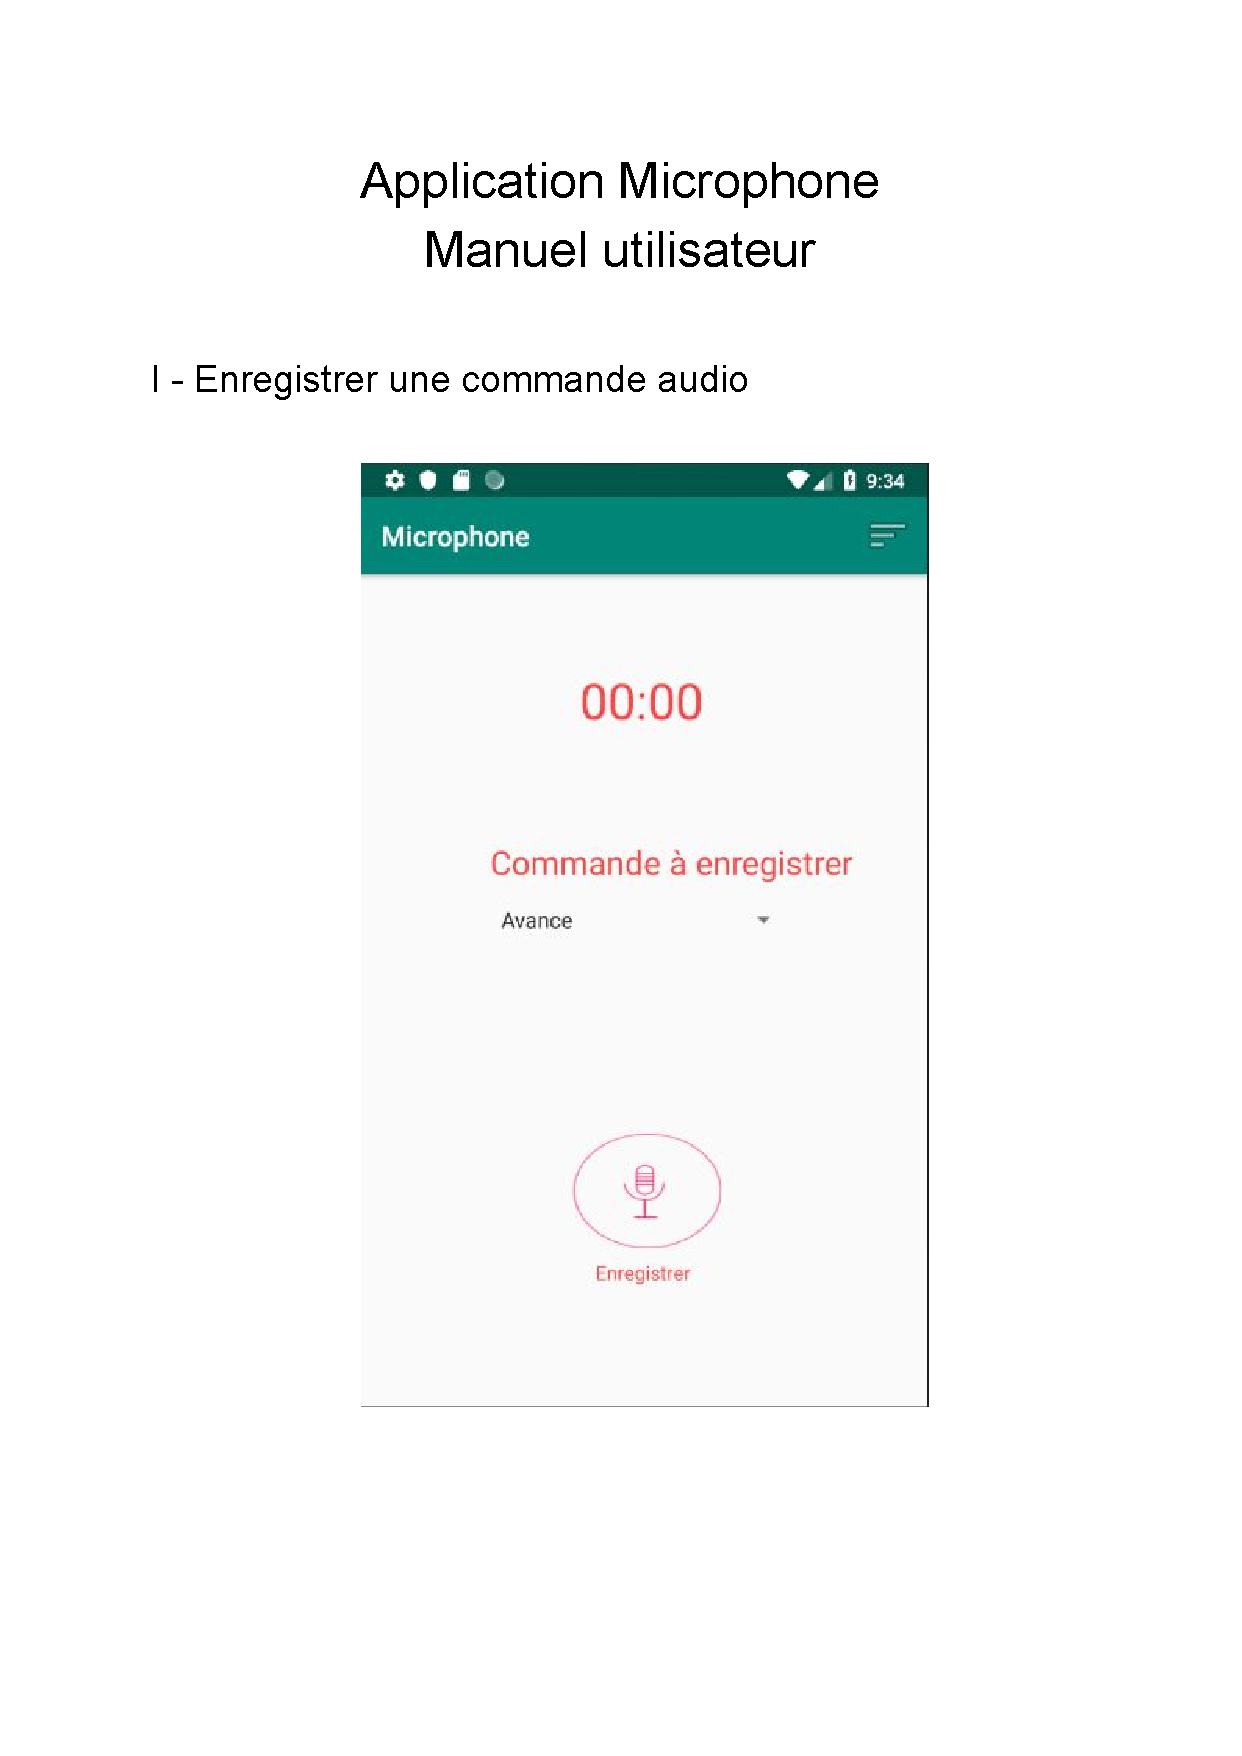
\includepdf[pages = 1-7]{Manuel-Utilisateur.pdf}
 

\end{document}


 
\end{apendix}

